\documentclass[tikz]{standalone}
\usepackage[utf8]{inputenc}
\usepackage{amsmath}
\usetikzlibrary{calc,positioning,shapes.multipart,arrows.meta}

\begin{document}
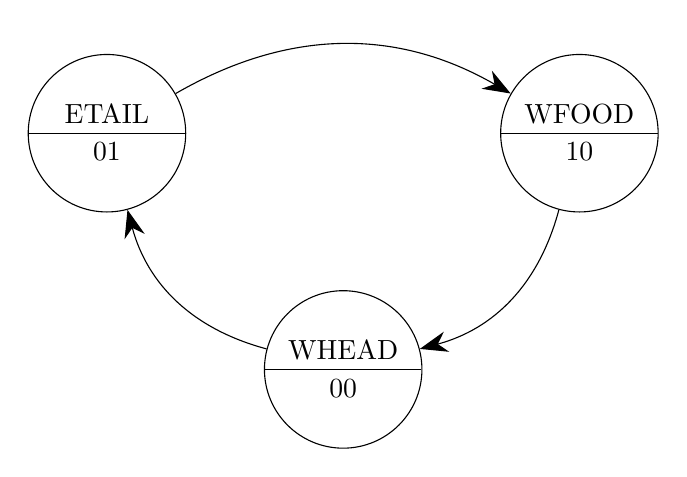
\begin{tikzpicture}
    \node[draw,circle split,minimum width=2cm] (etail) at (-3,0)
        {ETAIL \nodepart{lower} $01$};
        
    \node[draw,circle split,minimum width=2cm] (whead) at (0,-3) 
        {WHEAD \nodepart{lower} $00$}
        edge [-{Stealth[length=10]},bend left=30]
        node[auto] {} (etail);
    
    \node[draw,circle split,minimum width=2cm] (wfood) at (3,0) 
        {WFOOD \nodepart{lower} $10$}
        edge [{Stealth[length=10]}-,bend right=30]
        node[auto] {} (etail)
        edge [-{Stealth[length=10]},bend left=30]
        node[auto] {} (whead);
\end{tikzpicture}

\end{document}